\documentclass[output=paper,colorlinks,citecolor=brown]{langscibook}
\ChapterDOI{10.5281/zenodo.14266347}
    
\author{Masoud Mohammadirad\orcid{0000-0002-8531-5524}\affiliation{University of Cambridge}}
\title{Zagros region: The Kurdish-Gorani continuum}
\abstract{This chapter investigates the word order configuration of three Kurdic dialects confined within the Zagros mountains of western Iran: Gorani Gawraǰu\il{Gorani!Gawraǰu}; Central Kurdish  Sanandaj; Southern Kurdish Bijar.\il{Kurdish (Southern)!Bijar} These dialects share the commonality of having OV and Verb-Goal in their constituent ordering. However, the Gorani epicentre is characterised by extending post-predicate placement to Addressees, light-verb complements, and Locational complements in copular clauses. It will be argued that Central Kurdish dialects with post-predicate tendency for the above-mentioned constituents reflect a Gorani substrate.}

%move the following commands to the ``local...`` files of the master project when integrating this chapter
% \usepackage{tabularx}
% \usepackage{langsci-optional}
% \usepackage{langsci-gb4e}
% \usepackage{enumitem}
% \bibliography{localbibliography}
% \newcommand{\orcid}[1]{}
% \let\eachwordone=\itshape

\IfFileExists{../localcommands.tex}{
 \addbibresource{../collection_tmp.bib}
 \addbibresource{../localbibliography.bib}
 % add all extra packages you need to load to this file

\usepackage{tabularx,multicol}
\usepackage{url}
\urlstyle{same}

\usepackage{listings}
\lstset{basicstyle=\ttfamily,tabsize=2,breaklines=true}

\usepackage{langsci-basic}
\usepackage{langsci-optional}
\usepackage{langsci-lgr}
\usepackage{langsci-osl}
% \usepackage{./langsci/styles/langsci-lgr}
% \usepackage{./langsci/styles/langsci-osl}
% \usepackage{langsci-gb4e}

\usepackage{tikz}
\usetikzlibrary{patterns,calc}
\pgfdeclarepatternformonly{south east lines}{\pgfqpoint{-0pt}{-0pt}}{\pgfqpoint{3pt}{3pt}}{\pgfqpoint{3pt}{3pt}}{
    \pgfsetlinewidth{0.6pt}
    \pgfpathmoveto{\pgfqpoint{0pt}{3pt}}
    \pgfpathlineto{\pgfqpoint{3pt}{0pt}}
    \pgfpathmoveto{\pgfqpoint{.2pt}{-.2pt}}
    \pgfpathlineto{\pgfqpoint{-.2pt}{.2pt}}
    \pgfpathmoveto{\pgfqpoint{3.2pt}{2.8pt}}
    \pgfpathlineto{\pgfqpoint{2.8pt}{3.2pt}}
    \pgfusepath{stroke}}
    
\usepackage{stmaryrd}
\usepackage{wasysym}
\usepackage{multirow}
\usepackage{caption}
\usepackage{subcaption}
\usepackage{mathrsfs}
\usepackage{qtree}

\usepackage{linguex}


 %pminos do not split footnotes
% \interfootnotelinepenalty=10000 %Footnote in Laporte chapters has to be split SN


%\DeclareIndexNameFormat{default}{%
%\nameparts{#1}%
%\usebibmacro{index:name}%
%{\index[names]}%
%{\namepartfamily}%
%{\namepartgiveni}%
% {}% L1
% {}% L2
%{\namepartprefix}% generates spurious space L3
%{\namepartsuffix}% generates spurious space L4
%}

%  {\DeclareIndexNameFormat{default}{%
%     \usebibmacro{index:name}{\index[names]}{#1}{#3}{#5}{#7}}}

%\DeclareIndexNameFormat{default}{%
%  \usebibmacro{index:name}{\sindex[nom]}{#1}{#3}{#5}{#7}}

%\DeclareIndexNameFormat{default}{%
%  \usebibmacro{index:name}{\sindex[person]}{#1}{#3}{#5}{#7}}
%\DeclareIndexNameFormat{default}{%
%\nameparts{#1} \usebibmacro{index:name}{\sindex[person]]}{\namepartfamily}{‌​\namepartgiven}{\nam‌​epartprefix}{\namepa‌​rtsuffix}}

%\newcommand{\smiley}{:)}

%\renewbibmacro*{index:name}[5]{%
%\usebibmacro{index:entry}{#1}%
%{\iffieldundef{usera}{}{\thefield{usera}\actualoperator}\mkbibindexname{#2}{#3}{#4}{#5}}}

% \newcommand{\noop}[1]{}

%remove for final
%\overfullrule=1mm

\newcommand{\tobi}[2]}}
\renewcommand{\S}[1]{\tobi{#1}{\textsc{*}}}

% this volume references
% puts: [this volume]
% already defined: \citetv
%\newcommand{\citepv}[1]{(\citeauthor{#1} \citeyear*{#1} [this volume])}
\newcommand{\citealtv}[1]{\citeauthor{#1} \citeyear*{#1} [this volume]}

%parentheses around example number
\newcommand{\pref}[1]{(\ref{#1})}

% in-text examples

\newcommand{\lnex}[1]{\textit{#1}} %target lang word
\newcommand{\lnlit}[1]{(lit.: `#1')} %literal reading
\newcommand{\lnlat}[1]{(#1)} % latinization
\newcommand{\lntrans}[1]{`#1'} %translation
\newcommand{\lnexl}[2]%
{\lnex{#1}{} \lnlat{#2}} % ex with latinization
\newcommand{\lnexlat}[3]{\lnex{#1}{} \lnlat{#2}{} \lntrans{#3}} % ex with latinization and tranl.

%ch01
\newcommand{\co}[1]{\mbox{\textbf{#1}}}

%ch09

\newcommand{\cyrbulg}[1]{\begin{otherlanguage*}{bulgarian}#1\end{otherlanguage*}}


%ch10
\newcommand{\nlp}{{\small NLP}}
\newcommand{\mwe}{{\small MWE}}
\newcommand{\rae}{{\small RAE}}
\newcommand{\lvc}{{\small LVC}}
\newcommand{\pos}{{\small P}o{\small S}}
%\newcommand{\todo}[1]{ \textcolor{red}{#1} }

%\renewcommand{\labelenumi}{\theenumi}
%\ainamefmt{{vv}{ll}{, ff}{, jj}} % fullname

\newcommand{\biberror}[1]{{\color{red}#1}}

\newcommand{\osenovaitem}{--~}
 %% hyphenation points for line breaks
%% Normally, automatic hyphenation in LaTeX is very good
%% If a word is mis-hyphenated, add it to this file
%%
%% add information to TeX file before \begin{document} with:
%% %% hyphenation points for line breaks
%% Normally, automatic hyphenation in LaTeX is very good
%% If a word is mis-hyphenated, add it to this file
%%
%% add information to TeX file before \begin{document} with:
%% %% hyphenation points for line breaks
%% Normally, automatic hyphenation in LaTeX is very good
%% If a word is mis-hyphenated, add it to this file
%%
%% add information to TeX file before \begin{document} with:
%% \include{localhyphenation}
\hyphenation{
    Beck-man
    Ngu-yen
    back-chan-nel
    back-chan-nels
    mo-not-o-nous
    ste-reo-typ-i-cal
}

\hyphenation{
    Beck-man
    Ngu-yen
    back-chan-nel
    back-chan-nels
    mo-not-o-nous
    ste-reo-typ-i-cal
}

\hyphenation{
    Beck-man
    Ngu-yen
    back-chan-nel
    back-chan-nels
    mo-not-o-nous
    ste-reo-typ-i-cal
}

%  \boolfalse{bookcompile}
%  \togglepaper[5]%%chapternumber
}{}


\begin{document}
\begin{sloppypar}
    
\maketitle\label{WOWA:ch:9}

\section{Introduction}
This chapter investigates the \isi{word order} profiles of three Kurdic varieties spoken in the mountainous Zagros regions of Western Iran. The term Kurdic here refers both to the varieties that are “linguistically” considered Kurdish, i.e. Central Kurdish, Southern Kurdish, and Northern Kurdish and to the closely related but genetically more divergent languages Gorani and Zazaki\il{Zazaki} that are considered Kurdish in the broader ethnic and socio-cultural sense of the term. The Kurdish languages belong to the North-western branch of Iranian languages, along with Taleshi, Tati, Mazandarani, Balochi and others. 

The Kurdic varieties investigated in this study include the following: Gorani Gawraǰu,\il{Gorani!Gawraǰu} Central Kurdish of Sanandaj region, and Southern Kurdish Bijar.\il{Kurdish (Southern)!Bijar} These dialects are representative of Kurdic languages in Western Iran—and at least in the case of the Central Kurdish dialect spoken around Sanandaj — previous scholarship has identified a greater degree of influence from Gorani than in other varieties of Kurdish (see below). This chapter focuses on \isi{word order} and considers the possible effects of Gorani on this domain of syntax. To better assess the extent of Gorani influence, we will also consider three additional varieties as control languages: Hawrami Takht, a representative of a more conservative variety of Gorani, and two varieties of Central Kurdish, Mukri and Bingird, as representatives of Kurdish varieties outside immediate Gorani influence. \figref{Kurdish:fig:1} illustrates the localities in which these varieties are spoken.

% \setlength{\footheight}{49.46017pt} 
\largerpage

\begin{figure}
    \includegraphics[width=\textwidth]{figures/Gorani_fig1.jpeg}
    \caption{Investigated Kurdic dialects and control languages}
    \label{Kurdish:fig:1}
\end{figure}

The investigated dialects are situated at the intersection of Southern Kurdish and Central Kurdish-speaking areas. This intersection zone was once the Gorani heartland, which has since contracted to the mountainous Hawraman region and a few pockets across the region. There are accounts of \isi{language shift} from Gorani to Kurdish in the Sanandaj region (see §4). This motivates studying the doculects in this region to see what the effects of such an assumed shift are on the \isi{word order} profile of individual Central Kurdish dialects and whether it has any bearing on the classification of Central Kurdish dialects. There are now studies tackling this second aspect: \citet{mohammadirad_bound_nodate} is a study of the organisation of \isi{inflectional paradigm} in the periphery of the verb within Central Kurdish dialects. The author shows that the Southern Central Kurdish dialects adopt the Gorani pattern of (bound) \isi{argument} ordering in the verbal periphery, whereas the Northern Central Kurdish dialects opt for the opposing ordering. \citet{mohammadirad_gorani_inpress} is a case study of the Gorani \isi{substrate} features in the Central Kurdish dialect of the Sanandaj area across the whole grammar. The choice of the three doculects for this study is also motivated by the fact that Kurdic vernaculars in this region have remained unstudied with respect to their \isi{word order} properties (see §2). 

The Gorani \isi{substrate} hypothesis will be explored further in §4. It will be seen that the Gorani \isi{substrate} can explain some of the differences in \isi{word order} configuration in this region, which has contributed to a north/south continuum in Central Kurdish \isi{word order}. The northern half concerns the Mukri and Erbil dialects (to which Southern Kurdish Bijar\il{Kurdish (Southern)!Bijar} matches in \isi{word order}). In \isi{contrast}, the southern half is relevant for the Gorani zone of influence and contains the Central Kurdish Sanandaj\il{Kurdish (Central)!Sanandaj} (and possibly neighbouring Southern Kurdish varieties). Nonetheless, it should be noted that the number of data points, i.e., doculects, for this study is low, leading to the tentative nature of conclusions. 

 The Kurdish dialect of Bijar, also labelled Garrousi, lies at the northernmost edge of the Southern Kurdish speech zone. It is adjacent to Central Kurdish Mukri\il{Kurdish (Central)!Mukri} dialects to the northwest, Sanandaj-type Central Kurdish dialects to the southwest, and Azeri Turkish\il{Turkic!Azeri} dialects to the east. Earlier works on the Southern Kurdish dialect\il{Kurdish (Southern)!Bijar} of Bijar include small grammatical notes in \citet{de_morgan_mission_1904} and \citet{Fattah2000}, and a vocabulary list in \citet{querry_dialecte_1896}. It is assumed that the Southern Kurdish Bijar\il{Kurdish (Southern)!Bijar} is the result of migration from around Ilam, situated further to the south in Zagros mountains \citep[18]{Fattah2000}{}. 
 
Gawraǰu is a small village in the north of Kermanshah, western Iran, since destroyed due to a dam building in the region. Its Gorani dialect has been described in \citet{mahmoudveysi_gorani_2012}, and especially in \citet{bailey_grammar_2018}. The dialect is at the periphery of Gorani dialects and has been Kurdicised to a great degree; for instance, nominal case and gender marking are lost in Gorani Gawraǰu,\il{Gorani!Gawraǰu} contrary to the more conservative Gorani dialects.

The Kurdish dialect of the Sanandaj area is one of the southernmost dialects of Central Kurdish. The dialect is generally referred to as Ardalani when referring to the vernacular of Sanandaj itself and Laylakhi when referring to the vernaculars to the east of the Sanandaj region. Earlier work on Central Kurdish Sanandaj\il{Kurdish (Central)!Sanandaj} is restricted to \citegen{de_morgan_mission_1904} grammatical notes. More recently, the dialect has been described in more detail within the \isi{language contact} setting in Sanandaj \citep[][]{khan_language_2023}{}{}.

The data for all three dialects are from unscripted spoken narratives that were collected by the author (in the case of Kurdish Sanandaj and Kurdish Bijar) or imported from existing studies in the case of Gorani of\il{Gorani!Gawraǰu} Gawraǰu. The recordings were transcribed, translated, and analysed using the WOWA framework (\citetv{chapters/1_Haigetal_Intro}); see \tabref{Gorani:tab:1} for an overview of sources and corpus size.

\begin{table}
    \begin{tabularx}{\textwidth}{l@{}rrrQ}%p{.15\textwidth}p{.26\textwidth}}
\lsptoprule
&& \textbf{Total} & \textbf{Analysed} &  \\
\textbf{Doculect} & \textbf{Speakers} & \textbf{tokens}& \textbf{tokens}& \textbf{Source}\\
\midrule
CK Sanandaj & 8 & 1199 & 1180 & \citealt{mohammadirad_Sanandaj_Kurdish_2022}  \\
SK Bjiar & 3 & 1187 & 1150 & \citealt{mohammadirad_Bijar_Kurdish_2022}   \\
G Gawraǰū & 3 & 1325 & 1015 & \citealt{mohammadirad_gorani_2022} based  on \citealt{mahmoudveysi_gorani_2012}; \citealt{bailey_grammar_2018}  \\
\lspbottomrule
    \end{tabularx}
    \caption{Datasets from the WOWA corpus discussed in this chapter}
    \label{Gorani:tab:1}
\end{table}

The chapter pursues two main objectives: (i) an overview of post-predicate syntax in a sample of three doculects from the Zagros region. (ii) arguing for a Gorani \isi{substrate} as an explanation for some of the differences found in this region, which has contributed to a north/south continuum in Central Kurdish \isi{word order}. Applying a gradient corpus-based approach, this paper showcases the effect of \isi{language shift} through Gorani \isi{substrate} in contributing to the formation of a north/south continuum in the \isi{word order} profile of the Central Kurdish dialects. More precisely, I suggest that the shift from Gorani to Kurdish and/or high \isi{bilingualism} in Gorani in the Sanandaj region has led the Central Kurdish dialect of Sanandaj to be strikingly different in some of the post-predicate syntax from the Central Kurdish dialects in the North, e.g. Mukri. It should be noted, though, that the status of Gorani Gawraǰu\il{Gorani!Gawraǰu} is hard to reconcile with point (ii). As will be seen in \S\ref{MGKC:sec.areal}, it has been Kurdicised to a large degree and cannot be regarded as an assumed original state of a Gorani dialect once spoken in the region. 

This chapter is structured as follows. \S\ref{MGKC: sec.2} gives an overview of the literature on post-predicate arguments across Kurdish. \S\ref{sec: param} classifies major \isi{word order} parameters across the three investigated Kurdic dialects. \S\ref{MGKC:sec.areal} outlines areal issues in the configuration of certain \isi{word order} profiles. \S\ref{MFKC: sec.conc} is the conclusion.


\section{Previous scholarship on post-predicate arguments in Kurdish} \label{MGKC: sec.2}

\citet{haig_verb-goal_2015} is the first study on the ordering of ``Goals'' across Kurdish dialects in the context of contact with the north-eastern branch of Neo-Aramaic\il{Neo-Aramaic (NENA)} dialects, commonly called NENA. In \citeauthor{haig_verb-goal_2015}'s earlier (\citeyear{haig_verb-goal_2015}) terminology, ``Goal''  was used as a cover term encompassing human and non-human arguments of verbs of movement, recipients of verbs of \isi{transfer}, and Addressees of verbs of speech. These are all constituents that share ``\isi{endpoint semantics}.''\footnote{In more recent work, the inclusive use of the term `\isi{Goal}' has been abandoned, and `\isi{Goal}' is reserved exclusively for endpoint arguments of verbs of movement (see \citetv{chapters/1_Haigetal_Intro}).} Haig concludes that all Kurdish varieties share the commonality of post-predicate realisation of goals of verbs of movement and recipients of the verb `give,' a \isi{head-initial} trait which may be linked to an earlier imprint of Aramaic on Kurdish languages in their formative stages.

The main distinction between Kurdish dialects, according to Haig, is in finer-grained differences regarding the placement of Addressees (see also \citealt[]{Haig2017Keynote}) and beneficiaries. Haig makes the important observation that post-predicate Goals\is{Goal!post-verbal} are more prevalent across Kurdish dialects where there is a greater intensity of NENA speaking communities.\footnote{This is now statistically demonstrated in a recent study \citep[][]{haig_which_2023}{}{}: The Northern Kurdish dialect\il{Kurdish (Northern)!Ankara} spoken in Ankara shows less tendency for post-predicative realisation of Goals than Kurdish varieties in the immediate contact zone with NENA dialects.} Thus, within Northern Kurdish, the dialects to the south-east of Anatolia/northern Iraq, which have been in close contact with vernaculars of NENA for centuries, show more post-predicate realisation than Zazaki\il{Zazaki} and other Kurdish varieties in Central Anatolia, which show \isi{contact influence} from Turkish\il{Turkic!Turkish} and \il{Armenian} Armenian, and have the basic pattern of pre-predicate positioning for Addressees of verbs of speech. More recent research on larger samples from Kurdish and neighbouring languages has confirmed the preferred post-verbal placement of goals of verbs of motion and recipients, but some of the details regarding other roles have been revised in the light of additional data, see \citet{Haig2022PostPredicateCon}, \citetv{chapters/1_Haigetal_Intro}, and \sectref{sec: param} below.

\begin{sloppypar}
A relevant publication is \citegen{asadpour_typologizing_2022} dissertation on \isi{word order} variation within Kurdish languages in north-western Iran in contact with non-Iranian languages Neo-Aramaic\il{Neo-Aramaic}, \il{Armenian} and Turkic\il{Turkic}. \citet{asadpour_word_2022} is another work on \isi{word order} variation in Kurdish. His paper focuses on ``incorporated targets'' in the Mukri variety of Central Kurdish. By incorporated targets, the author means Goal-like arguments that appear between the constituting elements of a complex predicate, namely the non-verbal element and the light verb, for example, \textit{min} `\textsc{1sg}' in \textit{wiɫām=ī min=ī dā-w=a} [answer=\textsc{ez} \textsc{1sg=3sg:A} give\textsc{.pst-ptcp=perf}] `He gave an answer to me.' The author concludes that the variant ordering of incorporated targets in Mukri is accounted for by factors such as \isi{animacy} and length, which favour the preverbal position. 
\end{sloppypar}
In short, previous scholarship has mainly taken a broader perspective on the effects of \isi{language contact} on the \isi{word order} profile of Kurdish. Central Kurdish dialects, in general, and especially the Gorani zone of influence corresponding to the south of Central Kurdish speech zone, have remained understudied with regard to their \isi{word order} properties. Given this background, this chapter attempts to provide a more focused case study of \isi{language contact} and \isi{word order} within Kurdish, in particular, the southeasterly periphery. 

\section{Word order parameters} \label{sec: param}
Barring a few features, e.g., \isi{OV} order, the \isi{word order} parameters across the investigated dialects are predominantly \isi{head-initial}. 

\subsection{Adjective/noun}
In the investigated dialects, attribution in the noun phrase is formed by placing the \isi{adjective} following the head noun through a sort of head-marking formative called ezafe, which has different forms depending on the status of the head noun being indefinite (1.a-1.b)\footnote{Alternatively, the \isi{adjective} can be linked to the head noun through juxtaposition, e.g., Southern Kurdish Bijar\il{Kurdish (Southern)!Bijar} \textit{usāswār xās-ē} `a good horse-riding master' \citep[D, 0285]{mohammadirad_Bijar_Kurdish_2022}.}, or definite (1.c)\footnote{The ezafe particle \textit{=a}, generally dubbed ``compound ezafe,'' is a feature of all Central Kurdish, Southern Kurdish, and Gorani dialects but absent in the majority of Northern Kurdish dialects \citep[cf.][83]{mackenzie_kurdish_1962}.}

\ea
\ea\label{MGKC:ex:1a}
Gorani Gawraǰu \il{Gorani!Gawraǰu}(\citealt[E, 0770]{mohammadirad_gorani_2022}) \\
\gll žan=e ǰwān-ēk \\
woman\textsc{=ez} young\textsc{-indf} \\
\glt `a young woman'
\ex\label{MGKC:ex:1b}
Southern Kurdish Bijar \il{Kurdish (Southern)!Bijar}(\citealt[B, 0166]{mohammadirad_Bijar_Kurdish_2022}) \\
\gll sag=e sīya=y zil-aka-y \\
dog\textsc{=ez} black\textsc{=ez} big\textsc{-spec-indf} \\
\glt `a big black dog' \\
\ex\label{MGKC:ex:1c}
Central Kurdish Sanandaj \il{Kurdish (Central)!Sanandaj}(\citealt[A, 0065]{mohammadirad_Sanandaj_Kurdish_2022}) \\
\gll kanīšk=a gawra-(a)ka \\
girl\textsc{=ez} old-\textsc{def} \\
\glt `the older girl' \label{MGKC:ex:1d}
\z
\z 

While the default pattern remains \isi{head-initial} in adjective-noun constructions, these dialects show minor traces of \isi{head-final} syntax in a few closely-knit compound NPs. Here, the ezafe linker appears on the \isi{adjective} and has the form of \textit{=a} similar to (\ref{MGKC:ex:1d}):
\ea
Gorani Gawraǰu, Central Kurdish Sanandaj, and Southern Kurdish Bijar \il{Kurdish (Southern)!Bijar}\il{Kurdish (Central)!Sanandaj}\il{Gorani!Gawraǰu} \\
\gll juwān=a žin \\
beautiful\textsc{=ez} woman \\
\glt `beautiful woman' 
\z 

\subsection{Possessor/possessed}
In the investigated dialects, the structure of \isi{possessive} constructions is possessed first, possessor second. The unmarked pattern for linking the possessor to the possessed noun is through simple juxtaposition in Gorani Gawraǰu\il{Gorani!Gawraǰu} and Central Kurdish Sanandaj,\il{Kurdish (Central)!Sanandaj} but via ezafe linker in Southern Kurdish Bijar:\il{Kurdish (Southern)!Bijar}
\ea
\ea\label{MGKC:ex:3a}
Gorani Gawraǰu \il{Gorani!Gawraǰu}(\citealt[A, 0175]{mohammadirad_gorani_2022}) \\
\gll dim pišī-aka \\
tail cat-\textsc{def} \\
\glt `the tail of the cat'
\ex\label{MGKC:ex:3b}
Central Kurdish Sanandaj \il{Kurdish (Central)!Sanandaj}(\citealt[G, 0714]{mohammadirad_Sanandaj_Kurdish_2022}) \\
\gll kanīšk pāwšā \\
daughter king \\
\glt `the king's daughter' \\
\ex\label{MGKC:ex:3c}
Southern Kurdish Bijar \il{Kurdish (Southern)!Bijar}(\citealt[D, 0318]{mohammadirad_Bijar_Kurdish_2022}) \\
\gll zārū=ē pādišā=y maymün-ān \\
child\textsc{=ez} king\textsc{=ez} monkey\textsc{-pl} \\
\glt `the child of the king of monkeys'
\z
\z 

\subsection{Demonstrative/noun}
In all the three dialects, the demonstrative attributives are discontinuous: they consist of the demonstrative attributes, sensitive to distance distinction, to the left of the head noun, and the invariable deictic form \textit{=a} which attaches to the rightmost boundary of the NP, see \tabref{MGK:tab:2} for Gorani forms. Thus, the order of demonstrative plus the head noun cannot be readily classified as fitting into either \isi{head-initial} or \isi{head-final} syntax.

\begin{table}
    \begin{tabular}{lll}
\lsptoprule
 & \textbf{Proximal} & \textbf{Distal} \\
\midrule
\textsc{sg/pl} & \textit{ī …… a} &\textit{ā …… a}    \\
\lspbottomrule
    \end{tabular}
    \caption{Demonstrative attributes in Gorani Gawraǰu (\citealt[169]{bailey_grammar_2018}{}, simplified)}
    \label{MGK:tab:2}
\end{table}

\ea
\ea\label{MGKC:ex:4a}
Gorani Gawraǰu \il{Gorani!Gawraǰu}(\citealt[B, 0334]{mohammadirad_gorani_2022}) \\
\gll ī bizin=a \\
\textsc{dem.prox} goat=\textsc{deic} \\
\glt `this goat'
\ex\label{MGKC:ex:4b}
Gorani Gawraǰu \il{Gorani!Gawraǰu}(\citealt[170]{bailey_grammar_2018}) \\
\gll ā kār-ān=a \\
\textsc{dem.dist} task\textsc{-pl=deic} \\
\glt `those tasks' \\
\z
\z 

\subsection{Numeral/noun}
The investigated varieties share the commonality of ordering the numerals before head nouns. Morphologically, the head noun does not show number agreement with numerals above `one.' Examples:
\ea
\ea\label{MGKC:ex:5a}
Gorani Gawraǰu \il{Gorani!Gawraǰu}(\citealt[B, 0237]{mohammadirad_gorani_2022}) \\
\gll dü wačka \\
two offspring \\
\glt `two offsprings'
\ex\label{MGKC:ex:5b}
Central Kurdish Sanandaj \il{Kurdish (Central)!Sanandaj}(\citealt[A, 0001]{mohammadirad_Sanandaj_Kurdish_2022}) \\
\gll sē kuř \\
three son \\
\glt `three sons' \\
\ex\label{MGKC:ex:5c}
Southern Kurdish Bijar \il{Kurdish (Southern)!Bijar}(\citealt[H, 1148]{mohammadirad_Bijar_Kurdish_2022}) \\
\gll haš kīsa \\
eight sack \\
\glt `eight sacks'
\z
\z 

Taken together, in the investigated Kurdic languages, the structure of NP is DEM NUM N ADJ, e.g. Central Kurdish Sanandaj.\il{Kurdish (Central)!Sanandaj} \textit{aw sē kanīšk zarīf=a} [\textsc{dem.dist} three girl beautiful=\textsc{deic}] `those three beautiful girls.'

\subsection{Adpositions}
A mixed adpositional typology is a common feature of most Kurdish varieties. This is a reflection of their geographical distribution between \isi{OV} languages, e.g.\il{Armenian} Armenian, Turkic\il{Turkic}, Caucasian, and \isi{VO} languages, e.g. Arabic, Aramaic \citep[cf.][6--7]{stilo_circumpositions_2009}{}. The Kurdic dialects investigated here are no exception, though the levels of postpositionality differ significantly in these doculects (see \S\ref{MGKC:sect.summary}). Therefore, prepositions, postpositions, and circumpositions occur in these dialects. It is thus not straightforward to categorize these dialects easily into \isi{head-initial} vs. \isi{head-final} types.

\ea
\ea\label{MGKC:ex:6a}
Central Kurdish Sanandaj \il{Kurdish (Central)!Sanandaj}(\citealt[B, 0261]{mohammadirad_Sanandaj_Kurdish_2022}) \\
\gll bo šār \\
to town \\
\glt `to the town'
\ex\label{MGKC:ex:6b}
Central Kurdish Sanandaj \il{Kurdish (Central)!Sanandaj}(\citealt[A, 0010]{mohammadirad_Sanandaj_Kurdish_2022}) \\
\gll la kēf řaš=ā \\
in mountain black=\textsc{post} \\
\glt `at the black mountain' \\
\ex\label{MGKC:ex:6c}
Central Kurdish Sanandaj \il{Kurdish (Central)!Sanandaj}(\citealt[K, 1160]{mohammadirad_Sanandaj_Kurdish_2022}) \\
\gll das a-nē-t=a žin-ak(a)=aw\\
hand \textsc{ind}-put\textsc{.prs-3sg:A=drct} woman\textsc{-def=post} \\
\glt `She nudged the woman.'
\z
\z 

\subsection{Auxiliary/main verb}
Given the breadth of the subject, this section only deals with \isi{auxiliary} verbs in progressive constructions,\footnote{The more archaic auxiliaries, such as various forms of the verb `to be', are now univerbated with the lexical verb, and cannot be readily analysed as \isi{head-final} auxiliaries.} which precede the main verb, in \isi{contrast} to the tendency in \isi{OV} languages \citep[][100]{Dryer1992Greeburg}{}{}. 

\ea
\ea\label{MGKC:ex:7a}
Central Kurdish Sanandaj \il{Kurdish (Central)!Sanandaj}(\citealt[D, 0449]{mohammadirad_Sanandaj_Kurdish_2022}) \\
\gll xarīk=a jift a-kā \\
\textsc{aux=cop.3sg:S} plough \textsc{ind}-do.\textsc{prs.3sg:A} \\
\glt `He is ploughing.'
\ex\label{MGKC:ex:7b}
Gorani Gawraǰu \il{Gorani!Gawraǰu}(\citealt[43]{mahmoudveysi_gorani_2012}) \\
\gll tū hē=t kār ma-kar-ī \\
\textsc{2sg} \textsc{ptcl=2sg:A} work \textsc{ind}-do\textsc{.prs-2sg:A} \\
\glt `You are working.' \\
\z
\z 

\subsection{Complement clause/matrix verb}
The complement clause\is{complement!clause} follows the matrix verb in the investigated dialects. The complementation strategy is generally asyndetic without any connective particles. 

\ea
\ea\label{MGKC:ex:8a}
Southern Kurdish Bijar \il{Kurdish (Southern)!Bijar}(\citealt[F, 0848]{mohammadirad_Bijar_Kurdish_2022}) \\
\gll na-zānist ča kirdī=ya \\
\textsc{neg}-know.\textsc{pst.3sg:A} what do.\textsc{pst.ptcp.3sg:A=perf} \\
\glt `He didn't know what he had done.'
\ex\label{MGKC:ex:8b}
Central Kurdish Sanandaj \il{Kurdish (Central)!Sanandaj}(\citealt[D, 0444]{mohammadirad_Sanandaj_Kurdish_2022}) \\
\gll wā a-zān-ē a=y-xwā \\
\textsc{deic} \textsc{ind}-know.\textsc{prs-3sg:A} \textsc{ind=3sg:O-}eat.\textsc{prs.3sg:A} \\
\glt `He thought it (the wolf) would eat him.' \\
\ex\label{MGKC:ex:8c}
Gorani Gawraǰu \il{Gorani!Gawraǰu}(\citealt[C, 0396]{mohammadirad_gorani_2022}) \\
\gll ma-wīn-ē hüč nīya b-war-ē \\
\textsc{ind}-see\textsc{.prs-3sg:A} nothing \textsc{neg.cop.3sg:S} \textsc{sbjv}-eat\textsc{.prs-3sg:A} \\
\glt `He sees that there is absolutely nothing he may eat.'
\z
\z 

\subsection{Position of complementizer within the complement clause}
As remarked, \isi{complement} clauses are not usually introduced by complementizers. However, the corpus data shows that young, educated speakers tend to use the complementizer \textit{ki}, \textit{ka} in the initial position of some \isi{complement} clauses. Kurdic varieties thus pattern with \isi{VO} languages in this regard, as do all other Western Asian varieties of Iranian. 

\ea
\ea\label{MGKC:ex:9a}
Southern Kurdish Bijar \il{Kurdish (Southern)!Bijar}(\citealt[H, 1062]{mohammadirad_Bijar_Kurdish_2022}) \\
\gll zānist ki bār-a=y sangīn=a \\
know.\textsc{pst.3sg:A} \textsc{comp} load-\textsc{def=3sg:POS} heavy\textsc{=cop.3sg:S} \\
\glt `He (the man) knew that its (the donkey's) load was heavy.'

\ex\label{MGKC:ex:9b}
Central Kurdish Sanandaj \il{Kurdish (Central)!Sanandaj}(\citealt[B, 0278]{mohammadirad_Sanandaj_Kurdish_2022}) \\
\gll na=y-hēšt ka hamro-akān bi-diz-ē \\
\textsc{neg=3sg:A-}let\textsc{.pst} \textsc{comp} pear\textsc{-def.pl} \textsc{sbjv}-steal\textsc{.prs-3sg:A} \\
\glt `He didn't let him steal the pears.' \\
\ex\label{MGKC:ex:9c}
Gorani Gawraǰu \il{Gorani!Gawraǰu}(\citealt[424]{bailey_grammar_2018}) \\
\gll ni-m-wāz-ē ka bi-zān-ē \\
\textsc{neg-ind}-want\textsc{.prs-3sg:A} \textsc{comp} \textsc{sbjv-}know.\textsc{prs-3sg:A} \\
\glt `He doesn't want to know.'
\z
\z
\subsection{Nominal direct object/verb}
Kurdish languages are generally claimed to have basic \isi{OV} \isi{word order} (see \citealt[613]{Mccarus2009}{} and \citealt[51]{Opengin2016}{} for Central Kurdish; \citealt[672]{Fattah2000}{} for Southern Kurdish; \citealt[72]{mahmoudveysi_gorani_2013}{} for Gorani Zarda).\il{Gorani!Zarda} \tabref{Gorani:tab:3} summarizes the \isi{OV} ratio of nominal direct objects for each doculect.

\begin{table}
    \begin{tabularx}{\textwidth}{lrrr Yrr Yrr}
\lsptoprule
& \multicolumn{3}{c}{\textbf{G Gawraǰu}} & \multicolumn{3}{c}{\textbf{CK Sanandaj}} &  \multicolumn{3}{c}{\textbf{SK Bijar}}  \\
\cmidrule(lr){2-4}\cmidrule(lr){5-7}\cmidrule(lr){8-10}
 & \textbf{\textit{n}} & \textbf{n Po} & \textbf{Po} & \textbf{\textit{n}} & \textbf{n Po} & \textbf{Po} & \textbf{\textit{n}} & \textbf{n Po} & \textbf{Po}\\
\midrule
Direct \isi{object}&285&13&5\%&316&3&1\%&298&7&2\% \\
\lspbottomrule
    \end{tabularx}
    \caption{Frequencies of post-verbal (Po) nominal direct objects}
    \label{Gorani:tab:3}
\end{table}
It can be seen that Kurdic varieties are predominantly \isi{OV}, in line with the claims made in the literature. Nonetheless, it is noteworthy that Gorani Gawraǰu\il{Gorani!Gawraǰu} allows nominal direct objects to be placed after the verb at a relatively higher rate than Central Kurdish and Southern Kurdish. This might be a reflection of earlier contact between Gorani vernaculars and Semitic languages, such as Arabic and Aramaic. Note, however, that the absolute numbers of postverbal objects in Gorani Gawraǰu\il{Gorani!Gawraǰu} are very small (13). One might even consider a contact effect from Persian here. Post-verbal direct objects in Gorani are overwhelmingly definite (11 out of a total of 13 post-verbal objects) and could be reconciled with some notion of \isi{afterthought}.). In addition, they are usually arguments of the verb `lift, grasp,' which is then followed by the directional particle.\footnotemark 

\ea
\ea\label{MGKC:ex:10a}
Gorani Gawraǰu \il{Gorani!Gawraǰu}(\citealt[D, 0677]{mohammadirad_gorani_2022}) \\
\gll ānī ma-nam=ya quɫang \\
\textsc{3sg} \textsc{ind}-lift.\textsc{prs.3sg:A=drct} pickaxe \\
\glt `He (Farhad) grasps (lit. lift) the pickaxe.'
\ex\label{MGKC:ex:10b}
Gorani Gawraǰu \il{Gorani!Gawraǰu}(\citealt[D, 0685]{mohammadirad_gorani_2022}) \\
\gll tamāšā=m xās na-kard-ē ʕask-akān \\
looking=\textsc{1sg:A} well \textsc{neg}-do.\textsc{pst-ptcp} picture\textsc{-def.pl} \\
\glt `I have not looked very well at the pictures.' \\
\ex\label{MGKC:ex:10c}
Gorani Gawraǰu \il{Gorani!Gawraǰu}(\citealt[D, 0566]{mohammadirad_gorani_2022}) \\
\gll ma-wīn-ē ī dawrīš-a\\
\textsc{ind}-see.\textsc{prs-3sg:A} \textsc{dem.prox} dervish\textsc{-deic} \\
\glt `She sees this dervish.'
\z
\z 

\footnotetext{Likewise, a special \isi{VO} syntax is associated with the verb \textit{rāhištin} `to lift' in Kurmanji dialects. However, the issue seems to be more complicated in Gorani. In the closely related Hawrami  \il{Gorani!Hawrami} varieties, the verb \textit{namāy} `to lift' is intransitive, but its non-subject \isi{argument} always appears post-verbally. On the other hand, assuming that the directional particle in (\ref{MGKC:ex:10a}) flags a \isi{direct object}, then this could be linked to an Aramaic influence, as noted by Don Stilo (p.c). In \citegen{Khan2009JSana} description of the Neo-Aramaic dialect of Sanandaj, it is mentioned that a minor strategy for marking direct objects is to use an allative strategy. However, unlike Gorani, the \isi{direct object} precedes the verb. This could mean that the allative strategy for direct objects in Gorani and Kurdish is a secondary pattern borrowed from NENA but used for very specific/restricted contexts.}

The \isi{role} of \isi{definiteness} in licensing post-verbal objects in otherwise \isi{OV} languages has been noted in several contributions to this volume; for instance, in Persian, see \textcitetv{chapters/7_RasekhMahandetal_Persian} and \textcitetv{chapters/8_Parizadeh_ENP}. Given the overall low frequency of post-verbal objects, it is hard to make a generalization about the effect of humanness vs. non-humanness in the \isi{VO} configuration.

\subsection{Pronominal direct object/verb}
Similarly, \isi{OV} is the preferred order for free \isi{pronoun} direct objects; see examples in (\ref{MGKC:ex:11a}-\ref{MGKC:ex:11b}). Note that the number of tokens does not exceed 10 in each dataset, which precludes a premature conclusion on the \isi{word order} configuration of free pronouns. The main reason for the low frequency of free pronouns as direct objects seems to be that a \isi{direct object} is often indexed by a bound \isi{pronoun} in these languages, which is in complementary distribution with free pronouns. 

\ea 
\ea\label{MGKC:ex:11a}
Gorani Gawraǰu \il{Gorani!Gawraǰu}(\citealt[E, 0920]{mohammadirad_gorani_2022}) \\
\gll tu min=it kušt \\
\textsc{2sg} \textsc{1sg=2sg:A} kill.\textsc{pst}\\
\glt `You killed me.'
\ex\label{MGKC:ex:11b}
Southern Kurdish Bijar \il{Kurdish (Southern)!Bijar}(\citealt[D, 0457]{mohammadirad_Bijar_Kurdish_2022}) \\
\gll wāna san-ī \\
 \textsc{3pl} buy\textsc{.prs-3sg:A} \\
\glt `He buys them.' \\
\z
\z 

\subsection{Copula complements}
Complements of copular verbs show a high propensity to be placed pre-verbally. They exhibit less than 10\% of post-verbal realisation across three datasets (with Gorani having the highest rate of post-predicate copula complement\is{copula!complement}s due to semi-poetic language in one of the tales). At any rate, copula complement\is{copula!complement}s align with direct objects in having predominantly pre-predicate placement, as noted for all other \isi{OV} languages in the WOWA data set.
\ea
\ea\label{MGKC:ex:12a}
Central Kurdish Sanandaj \il{Kurdish (Central)!Sanandaj}(\citealt[B, 0543]{mohammadirad_Sanandaj_Kurdish_2022}) \\
\gll fra wiryā a-w-ē \\
very clever \textsc{ind}-be.\textsc{prs-3sg:S} \\
\glt `She was very clever.'
\ex\label{MGKC:ex:12b}
Gorani Gawraǰu \il{Gorani!Gawraǰu}(\citealt[C, 0524]{mohammadirad_gorani_2022}) \\
\gll ēma řafīq bīs-yām̄ \\
\textsc{1pl} friend be.\textsc{pst-1pl:S} \\
\glt `We were friends.' \\
\ex\label{MGKC:ex:12c}
Southern Kurdish Bijar \il{Kurdish (Southern)!Bijar}(\citealt[D, 0278]{mohammadirad_Bijar_Kurdish_2022}) \\
\gll žin-a=y dugīyān d-\=u \\
wife-\textsc{def=3sg:POS} pregnant \textsc{ind}-be.\textsc{prs.3sg:S} \\
\glt `His wife was pregnant.'
\z
\z 

\subsection{Goal/verb} \label{MGKC_goal}
\citet{haig_verb-goal_2015,Haig2022PostPredicateCon} suggests that within Kurdish goals of verbs of movement (e.g., `go,' `come') and goals of verbs of caused motion (e.g. `put,' `take') have the highest propensity to occur in the post-predicate position among \isi{endpoint} constituents. \tabref{MGKC:tab:4} exhibits the linear position of Goals and Caused goals relative to the verb.

\begin{table}
    \begin{tabularx}{\textwidth}{lrrrYrrYrr}
\lsptoprule
& \multicolumn{3}{c}{\textbf{G Gawraǰu}} & \multicolumn{3}{c}{\textbf{CK Sanandaj}} &  \multicolumn{3}{c}{\textbf{SK Bijar}}  \\
\cmidrule(lr){2-4}\cmidrule(lr){5-7}\cmidrule(lr){8-10}
 & \textbf{\textit{n}} & \textbf{n Po} & \textbf{Po} & \textbf{\textit{n}} & \textbf{n Po} & \textbf{Po} & \textbf{\textit{n}} & \textbf{n Po} & \textbf{Po}\\
\midrule
Goals (simple)&158&148&94\%&183&162&88\%&181&172&95\% \\
Goals (caused)&105&103&98\%&150&144&96\%&121&117&97\% \\
All Goals&263&251&96\%&333&306&92\%&302&289&96\% \\
\lspbottomrule
    \end{tabularx}
    \caption{Frequencies of post-verbal (Po) Goals in three Kurdic doculects}
    \label{MGKC:tab:4}
\end{table}

As can be seen from \tabref{MGKC:tab:4}, overall Goals show more than 90\% post-predicate realisation. This has been claimed to reflect the \isi{convergence} of these Kurdic dialects with Semitic languages \citep[cf.][]{haig_which_2023}{}{}. It is notable that Goals slightly lag behind Caused goals in post-predicate realisation. Pre-verbal Goal\is{Goal!pre-verbal}s in these varieties occur often with some notion of ``refined motion,'' which often expresses \isi{atelicity}, see (\ref{MGKC:ex:13a}), whereas caused goals express more clearly an \isi{endpoint} to the action of the verb, thus post-verbal, cf. (\ref{MGKC:ex:13b}).
\ea\label{MGKC:ex:13}
\ea\label{MGKC:ex:13a}
Southern Kurdish Bijar \il{Kurdish (Southern)!Bijar}(\citealt[H, 1128]{mohammadirad_Bijar_Kurdish_2022}) \\
\gll waraw samt=i bāzār du-řī-yā-n \\
to direction=\textsc{ez} bazaar \textsc{ipfv}-go.\textsc{pst-ipfv-3pl:S} \\
\glt `They were going in the direction of bazaar.'
\ex\label{MGKC:ex:13b}
Southern Kurdish Bijar \il{Kurdish (Southern)!Bijar}(\citealt[D, 0476]{mohammadirad_Bijar_Kurdish_2022}) \\
\gll siqān-a nīyā war saw=aw\\
bone-\textsc{def} put\textsc{.pst.3sg:A} front dog=\textsc{post} \\
\glt `She put the bone in front of the dog.' \\
\z
\z 

\subsection{Complements of `become'} \label{subs_become_cop}
Within the investigated Kurdic dialects, the \isi{inchoative} verb `become' has a special syntax. It implies a change of state, e.g. `He became a king.' The verb `become' has an identical morphology as `be,' but unlike the latter, the \isi{complement} of `become' is usually realised post-predicatively, if it is a NP. Adjective complements of `become,' on the other hand, are generally pre-verbal. The examples in (\ref{MGKC:ex:14}) illustrate the placement of nominal complements. It is notable that the nominal \isi{complement} of \isi{inchoative} `become' is flagged by the \isi{preposition} \textit{ba}, cf. (\ref{MGKC:ex:14b}), which can be and is often cliticised to the verb and glossed as DRCT (directional particle).

\ea\label{MGKC:ex:14}
\ea\label{MGKC:ex:14a}
Gorani Gawraǰu \il{Gorani!Gawraǰu}(\citealt[E, 0786]{mohammadirad_gorani_2022}) \\
\gll ma-sūz-ē ma-w-u xuɫ \\
\textsc{ind-}burn.\textsc{prs-3sg:S} \textsc{ind}-be.\textsc{prs-3sg:S} ash \\
\glt `It (the wood) has burned up (and) turned to ashes.'
\ex\label{MGKC:ex:14b}
Central Kurdish Sanandaj \il{Kurdish (Central)!Sanandaj}(\citealt[C, 0430]{mohammadirad_Sanandaj_Kurdish_2022}) \\
\gll bū ba šaw \\
become.\textsc{pst.3sg:S} into night \\
\glt `It turned night.' \\
\ex\label{MGKC:ex:14c}
Southern Kurdish Bijar \il{Kurdish (Southern)!Bijar}(\citealt[B, 112]{mohammadirad_Bijar_Kurdish_2022}) \\
\gll tā d-ū=a nīmarū \\
until \textsc{ind-}become\textsc{.prs.3sg:S=drct} noon \\
\glt `Until it became noon.'
\z
\z 
The reversed ordering for adjectival complements is exhibited in (\ref{MGKC:ex:15}):

\ea\label{MGKC:ex:15}
\ea\label{MGKC:ex:15a}
Gorani Gawraǰu \il{Gorani!Gawraǰu}(\citealt[B, 0220]{mohammadirad_gorani_2022}) \\
\gll āwis ma-w-u bizin-aka \\
pregnant \textsc{ind}-be.\textsc{prs-3sg:S} goat-\textsc{def} \\
\glt `The goat becomes pregnant.'
\ex\label{MGKC:ex:15b}
Central Kurdish Sanandaj \il{Kurdish (Central)!Sanandaj}(\citealt[C, 0370]{mohammadirad_Sanandaj_Kurdish_2022}) \\
\gll dang=ī nāzik=aw bū \\
voice=\textsc{3sg:POS} soft=\textsc{compl} be.\textsc{pst.3sg:S} \\
\glt `His voice became soft.' \\
\ex\label{MGKC:ex:15c}
Southern Kurdish Bijar \il{Kurdish (Southern)!Bijar}(\citealt[D, 405]{mohammadirad_Bijar_Kurdish_2022}) \\
\gll mas d-ū \\
drunk \textsc{ind}-be\textsc{.prs.3sg:S} \\
\glt `She becomes drunk.'
\z
\z 

\tabref{MGKC:tab:5} summarizes the linear positioning of complements of `become':

\begin{table}
    \begin{tabularx}{\textwidth}{lrrrYrrYrr}
\lsptoprule
& \multicolumn{3}{c}{\textbf{G Gawraǰu}} & \multicolumn{3}{c}{\textbf{CK Sanandaj}} &  \multicolumn{3}{c}{\textbf{SK Bijar}}  \\
\cmidrule(lr){2-4}\cmidrule(lr){5-7}\cmidrule(lr){8-10}
 & \textbf{\textit{n}} & \textbf{n Po} & \textbf{Po} & \textbf{\textit{n}} & \textbf{n Po} & \textbf{Po} & \textbf{\textit{n}} & \textbf{n Po} & \textbf{Po}\\
\midrule
N \isi{complement}& 14& 12& 86\%& 22& 22& 100\%& 14& 13& 93\% \\
Adj \isi{complement}& 20& 2& 10\%& 12& 1& 8\%& 17& 3& 18\% \\
All complements& 34& 14& 41\%& 34& 23& 68\%& 31& 16& 51\% \\
\lspbottomrule
    \end{tabularx}
    \caption{Frequencies of post-verbal (Po) complements of `become' in three Kurdic doculects}
    \label{MGKC:tab:5}
\end{table}

As can be seen in \tabref{MGKC:tab:5}, it is clear that adjectival complements of \isi{inchoative} `become' show strikingly less tendency than nominal complements to be realised post-predicatively. The reason lies perhaps in the fact that the \isi{adjective} is treated as the non-verbal \isi{complement} of `become'; hence, the combination Adjective + become acts more like a complex predicate, in which the placement of adjectives is fixed preverbally. In \isi{contrast}, the nominal complements are framed into a prepositional phrase and are treated like a Goal of verbs of movement.

\subsection{Recipient/verb}
Recipients of verbs of `giving' are next in line in the likelihood to appear in the post-predicate position. An important observation is that in all three varieties, nominal and/or free pronouns recipients are overwhelmingly post-predicate; see \tabref{MGKC:tab:6}.


\begin{table}[t]
\begin{tabularx}{\textwidth}{Qrrrrrrrrr}
\lsptoprule
& \multicolumn{3}{c}{\textbf{G Gawraǰu}} & \multicolumn{3}{c}{\textbf{CK Sanandaj}} &  \multicolumn{3}{c}{\textbf{SK Bijar}}  \\
\cmidrule(lr){2-4}\cmidrule(lr){5-7}\cmidrule(lr){8-10}
 & \textbf{\textit{n}} & \textbf{n Po} & \textbf{Po} & \textbf{\textit{n}} & \textbf{n Po} & \textbf{Po} & \textbf{\textit{n}} & \textbf{n Po} & \textbf{Po}\\
\midrule
 Non-bound recipients& 13& 13& 100\%& 9& 9& 100\%& 9& 9& 100\% \\
Bound recipients& 31& 31& 100\%& 26& 12& 46\%& 23& 0& 0\% \\
All recipients& 44& 44& 100\%& 35& 21& 60\%& 32& 9& 28\% \\
\lspbottomrule
    \end{tabularx}
    \caption{Frequencies of post-verbal (Po) recipients in three Kurdic doculects}
    \label{MGKC:tab:6}
\end{table}


In the investigated dialects, pronominal recipients often occur as \isi{clitic} pronouns, prosodically dependent on some other item. The dialects differ significantly in the positioning of these bound recipients; see \tabref{MGKC:tab:6}. They also differ in the syntax of these formatives. In Southern Kurdish Bijar\il{Kurdish (Southern)!Bijar} and Gorani Gawraǰu, bound recipients remain attached to their governing \isi{preposition} but never occur on the verb. However, in Central Kurdish Sanandaj,\il{Kurdish (Central)!Sanandaj} bound pronouns have a special syntax of their own in the present tense such that they are realized on the constituent preceding their governing head (see \citealt[]{Mohammadirad2020}{}; \citealt[]{opengin_pronominal_2022}{} for the grammar of bound pronouns within Kurdish).
\ea
\ea\label{MGKC:ex:16a}
Southern Kurdish Bijar \il{Kurdish (Southern)!Bijar}(\citealt[A, 0069]{mohammadirad_Bijar_Kurdish_2022}) \\
\gll mirw-aga xā \textbf{wa=y} da-y \\
hen-\textsc{def} egg to=\textsc{3sg:R} give\textsc{.prs-3sg:A} \\
\glt `The hen gives him egg.'
\ex\label{MGKC:ex:16b}
Central Kurdish Sanandaj \il{Kurdish (Central)!Sanandaj}(\citealt[I, 0990]{mohammadirad_Sanandaj_Kurdish_2022}) \\
\gll poɫ=o pē a-wa-m \\
money=\textsc{2sg:R} to \textsc{ind}-give\textsc{.prs-1sg:A} \\
\glt `I will give you money.' \\
\z
\z 

The following examples illustrate the post-verbal positioning of bound recipients:
\ea
\ea\label{MGKC:ex:17a}
Gorani Gawraǰu \il{Gorani!Gawraǰu}(\citealt[B, 0233]{mohammadirad_gorani_2022}) \\
\gll šīr-aka=š ma-t-ī=ya \textbf{wan=šān} \\
milk-\textsc{def=3sg:POS} \textsc{ind-}give.\textsc{prs-3sg:A=drct} to=\textsc{3pl:R} \\
\glt `She gives them her milk.'
\newpage
\ex\label{MGKC:ex:17b}
Central Kurdish Sanandaj \il{Kurdish (Central)!Sanandaj}(\citealt[B, 0323]{mohammadirad_Sanandaj_Kurdish_2022}) \\
\gll sē dāna hamro=y dā \textbf{pē=yān} \\
three \textsc{clf} pear=\textsc{3sg:A} give.\textsc{pst} to=\textsc{3pl:R} \\
\glt `He gave them three pears.' \\
\z
\z 


According to \tabref{MGKC:tab:6}, bound pronouns have different \isi{word order} preferences than nominals, except in Gorani Gawraǰu.\il{Gorani!Gawraǰu} The crucial point here is that in Gorani Gawraǰu,\il{Gorani!Gawraǰu} the \isi{adposition} itself occurs after the verb (and therefore the non-mobile \isi{clitic} with it). In \isi{contrast}, in Southern Kurdish Bijar,\il{Kurdish (Southern)!Bijar} the \isi{adposition} and the non-mobile \isi{clitic} appear pre-verbally. Likewise, in Central Kurdish Sanandaj,\il{Kurdish (Central)!Sanandaj} the \isi{adposition} remains preverbal, at least quite frequently. The different \isi{word order} preferences of nominal and bound recipients are indeed worthy of further research, especially that \citegen{hawkins_asymmetry_2008} typology of ``obliques'' only accounts for the \isi{word order} constellation of nominal constituents.

\subsection{Addressee/verb}
Discussing the \isi{word order} preferences of Addressees across Northern Kurdish, \citet{Haig2022PostPredicateCon} makes several important observations: (i) there is a correlation between the \isi{flagging} of the Addressee \isi{argument} and its position relative to the verb, such that post-predicate Addressees are not flagged via postpositions and/or circumpositions; (ii) Addressees of verbs which have \isi{telic} aspectual meanings, i.e. `say/tell' are more expected to occur post-predicatively than Addressees of a verb of speech which indicates non-\isi{telic} aspectual meaning, e.g. `speak,' the reason being that the former is associated with an \isi{endpoint} activity whereas the latter is not. Examples of the positionality of Addressee arguments are presented below, see \tabref{MGKC:tab:7} for percentages.
\ea
\ea\label{MGKC:ex:18a}
Central Kurdish Sanandaj \il{Kurdish (Central)!Sanandaj}(\citealt[G, 0660]{mohammadirad_Sanandaj_Kurdish_2022}) \\
\gll mard wit=ī=ya žin-aka=y \\
\textsc{pn} say\textsc{.pst=3sg:A=drct} wife\textsc{-def=3sg:POS} \\
\glt `Mard said to his wife.'
\ex\label{MGKC:ex:18b}
Gorani Gawraǰu \il{Gorani!Gawraǰu}(\citealt[A, 0079]{mohammadirad_gorani_2022}) \\
\gll m-wā=ya dāyka=y čīman \\
\textsc{ind}-say\textsc{.prs.3sg:A=drct} mother=\textsc{ez} \textsc{pn} \\
\glt `She says to the mother of Čiman.' \\
\ex\label{MGKC:ex:18c}
Southern Kurdish Bijar \il{Kurdish (Southern)!Bijar}(\citealt[A, 0004]{mohammadirad_Bijar_Kurdish_2022}) \\
\gll wa pišī-ya īš-ī\\
to cat-\textsc{def} say\textsc{.prs-3sg:A} \\
\glt `She says to the cat.'
\z
\z 

\begin{table}
\begin{tabularx}{\textwidth}{lrrrYrrYrr}
\lsptoprule
& \multicolumn{3}{c}{\textbf{G Gawraǰu}} & \multicolumn{3}{c}{\textbf{CK Sanandaj}} &  \multicolumn{3}{c}{\textbf{SK Bijar}}  \\
\cmidrule(lr){2-4}\cmidrule(lr){5-7}\cmidrule(lr){8-10}
 & \textbf{\textit{n}} & \textbf{n Po} & \textbf{Po} & \textbf{\textit{n}} & \textbf{n Po} & \textbf{Po} & \textbf{\textit{n}} & \textbf{n Po} & \textbf{Po}\\
\midrule
 Addressees of `say/tell' & 13 & 6 & 46\% & 13 & 13 & 92\% & 23 & 0 & 0\% \\
Addressees (total) & 25 & 10 & 40\% & 22 & 16 & 72\% & 52 & 2 & 4\% \\
\lspbottomrule
    \end{tabularx}
    \caption{Frequencies of post-verbal (Po) nominal Addressees of all verbs vs. nominal Addressees of `say/tell'}
    \label{MGKC:tab:7}
\end{table}

It is clear that Addressees in Central Kurdish Sanandaj\il{Kurdish (Central)!Sanandaj} and Gorani Gawraǰu are realised far more frequently rightward after the predicate than Addressees in the Southern Kurdish Bijar.\il{Kurdish (Southern)!Bijar} Note, however, that the rate of post-verbal Addressees in the latter remains near zero (only two tokens out of 52 have postverbal ordering). Thus, the preverbal position of Addressees in Southern Kurdish Bijar\il{Kurdish (Southern)!Bijar} is independent of the type of verb; it is a structural position. 

It is also notable that Addressees of `say/tell' statistically yield even more post-predicate tendency, reflecting that Addressees of `say/tell' are more clearly associated with the notion of \isi{endpoint} than verbs like `speak' \citep[cf.][359]{Haig2022PostPredicateCon}{}{}. 

As for the \isi{flagging} strategy, prepositional \isi{flagging} remains the primary mode of expressing Addressees across the dialects investigated here. Circumpositions rarely occur, and if they do, the pre-verbal position is the only option, in line with the tendency reported for Northern Kurdish in \citet{Haig2022PostPredicateCon}. 

\subsection{Place constituents}
Place constituents here refer to arguments which denote `static location' in clauses like `He works at a factory.'; see \tabref{MGKC:tab:8} for the rate of post-predicate place constituents.
\ea
\ea\label{MGKC:ex:19a}
Southern Kurdish Bijar \il{Kurdish (Southern)!Bijar}(\citealt[A, 0079]{mohammadirad_Bijar_Kurdish_2022}) \\
\gll la sar ay gūl=a mālāw-in \\
on top \textsc{dem.prox} pond=\textsc{deic} bathe.\textsc{prs-3pl:S} \\
\glt `They bathe at this pond.'
\ex\label{MGKC:ex:19b}
Central Kurdish Sanandaj \il{Kurdish (Central)!Sanandaj}(\citealt[A, 0012]{mohammadirad_Sanandaj_Kurdish_2022}) \\
\gll šaw la kēf řaš=ā na-xaf-in \\
night in mountain black=\textsc{post} \textsc{proh}-sleep.\textsc{prs-2pl:S} \\
\glt `Do not sleep the night in the black mountain!' \\
\newpage
\ex\label{MGKC:ex:19c}
Gorani Gawraǰu \il{Gorani!Gawraǰu}(\citealt[B, 0352]{mohammadirad_gorani_2022}) \\
\gll ča=tān waš ka(rd) a(ž) ka=y lālo\\
what=\textsc{2pl:A} good do\textsc{.pst} in house=\textsc{ez} uncle \\
\glt `What did you prepare in your uncle's house?'
\z
\z 

\begin{table}[t]
    \begin{tabularx}{\textwidth}{lrrrYrrYrr}
\lsptoprule
& \multicolumn{3}{c}{\textbf{G Gawraǰu}} & \multicolumn{3}{c}{\textbf{CK Sanandaj}} &  \multicolumn{3}{c}{\textbf{SK Bijar}}  \\
\cmidrule(lr){2-4}\cmidrule(lr){5-7}\cmidrule(lr){8-10}
 & \textbf{\textit{n}} & \textbf{n Po} & \textbf{Po} & \textbf{\textit{n}} & \textbf{n Po} & \textbf{Po} & \textbf{\textit{n}} & \textbf{n Po} & \textbf{Po}\\
\midrule
 Place arguments & 60 & 25 & 42\% & 115 & 20 & 17\% & 65 & 10 & 15\% \\
\lspbottomrule
    \end{tabularx}
    \caption{Frequencies of post-verbal (Po) nominal Addressees of all verbs vs. nominal Addressees of `say/tell'}
    \label{MGKC:tab:8}
\end{table}

Comparing the post-predicate realisation of place constituents to Goals (see \ref{MGKC_goal}) reveals that Goals differ significantly from Place constituents in post-verbal occurrence. Nevertheless, Place constituents are more post-posed than, say, direct objects, suggesting that the notion of `location,' whether \isi{endpoint} or not, triggers \isi{extraposition} in the Kurdic varieties of the Zagros region. 

\subsection{Place constituents of a copular verb} \label{subs-cop-loc}
Locational copula construction\is{copula!construction}
s are clauses in which the place constituent is a \isi{complement} of the copular verb, e.g. `I am at home.' In Central Kurdish Sanandaj\il{Kurdish (Central)!Sanandaj} and Gorani Gawraǰu, the predicate is an existential \isi{copula} in such constructions, which requires the place \isi{complement} to appear post-verbally. This existential construction is limited to the present tense, though; in the past tense, the past base of the verb `to be' is used as the predicate, and its \isi{complement} is generally realised preverbally. Southern Kurdish Bijar\il{Kurdish (Southern)!Bijar}, on the other hand, consistently puts the place constituent before the \isi{copula} verb; see \tabref{MGKC:tab:9} for percentages. \footnote{The high percentage of post-verbal place constituents of present \isi{copula} verbs might be an indication of Aramaic influence in the core Gorani speech zone (Don Stilo, p.c.). However, it is noticeable that in NENA Sanandaj, \isi{locative} complements of \isi{copula} verbs are by default realised pre-verbally (see \citealt[]{Khan2009JSana}).}

\ea
\ea\label{MGKC:ex:20a}
Gorani Gawraǰu \il{Gorani!Gawraǰu}(\citealt[G, 1306]{mohammadirad_gorani_2022}) \\
\gll zangoɫ=a ziřa hā pišt=e kanü \\
bell=\textsc{ez} swinging \textsc{exist.3sg:S} back=\textsc{ez} flour\_bin \\
\glt `The swinging bell is in the back of bin of flour.'
\ex\label{MGKC:ex:20b}
Central Kurdish Sanandaj \il{Kurdish (Central)!Sanandaj}(\citealt[K, 1071]{mohammadirad_Sanandaj_Kurdish_2022}) \\
\gll hā la māɫ-ē tārīk=ā \\
\textsc{exist.3sg:S} in house-\textsc{indf} dark=\textsc{post} \\
\glt `(He) is in a dark house.' \\
\ex\label{MGKC:ex:20c}
Southern Kurdish Bijar \il{Kurdish (Southern)!Bijar}(\citealt[D, 0397]{mohammadirad_Bijar_Kurdish_2022}) \\
\gll kēnī la pāl daryā d-ū\\
spring in side sea \textsc{ind-}be\textsc{.prs.3sg:S} \\
\glt `The spring is next to the sea.'
\z
\z 

\begin{table}[t]
    \begin{tabularx}{\textwidth}{lrrrYrrYrr}
\lsptoprule
& \multicolumn{3}{c}{\textbf{G Gawraǰu}} & \multicolumn{3}{c}{\textbf{CK Sanandaj}} &  \multicolumn{3}{c}{\textbf{SK Bijar}}  \\
\cmidrule(lr){2-4}\cmidrule(lr){5-7}\cmidrule(lr){8-10}
 & \textbf{\textit{n}} & \textbf{n Po} & \textbf{Po} & \textbf{\textit{n}} & \textbf{n Po} & \textbf{Po} & \textbf{\textit{n}} & \textbf{n Po} & \textbf{Po}\\
\midrule
 Place arguments& 6& 4& 66\%& 7& 7& 100\%& 11& 0& 0\% \\
\lspbottomrule
    \end{tabularx}
    \caption{Frequencies of post-verbal (Po) place arguments of present tense copula constructions in three Kurdic doculects}
    \label{MGKC:tab:9}
\end{table}

While the number of tokens is low and no categorial conclusions can be made, it is clear that the Kurdic varieties in the Gorani zone of influence have a clear tendency for post-verbal positioning of place arguments of copular verbs. In \isi{contrast}, Southern Kurdish Bijar\il{Kurdish (Southern)!Bijar} opts for an opposing tendency, namely preverbal placement. 

\subsection{Light verb complements} \label{subs_lvc}
In the Kurdic dialects investigated here, light verb complements of certain types of complex predicates appear after the light verb, e.g., Central Kurdish Sanandaj\il{Kurdish (Central)!Sanandaj} \textit{kaft=a řē} [fall.\textsc{pst.3sg:S=drct} road] `He set out.' In such predicates, the light verb is obligatorily followed by the directional \isi{clitic}. A variety of light verbs can be used in such constructions, e.g., `do,' `fall,' `come,' `sit,' `grab,' etc. It is notable that several of these light verbs involve motion verbs, e.g. `fall,' `come,' and the \isi{complement} can be considered a metaphorical \isi{Goal}. The light verbs used here can sometimes have an `inceptive' sense. 

\ea
\ea\label{MGKC:ex:21a}
Central Kurdish Sanandaj \il{Kurdish (Central)!Sanandaj}(\citealt[D, 484]{mohammadirad_Sanandaj_Kurdish_2022}) \\
\gll a-kaf-ēt=a xwašī=yā \\
\textsc{ind}-fall.\textsc{prs-3sg:S=drct} happiness=\textsc{post} \\
\glt `He will get rich. (Lit. He will fall into happiness)'
\ex\label{MGKC:ex:21b}
Gorani Gawraǰu \il{Gorani!Gawraǰu}(\citealt[A, 0061]{mohammadirad_gorani_2022}) \\
\gll hānī-aka m-ā=ya qisa \\
spring-\textsc{def} \textsc{ind}-come.\textsc{prs.3sg:S=drct} speech \\
\glt `The water spring starts to speak.' \\
\ex\label{MGKC:ex:21c}
Southern Kurdish Bijar \il{Kurdish (Southern)!Bijar}(\citealt[E, 677]{mohammadirad_Bijar_Kurdish_2022}) \\
\gll dāɫik=ī girt=ay=a bāwiš=aw\\
mother=\textsc{3sg:POS} grab.\textsc{pst.3sg:A=3sg:O=drct} hug=\textsc{post} \\
\glt `Her mother hugged her.'
\z
\z 

In a similar manner, in the Bahdini variety of Northern Kurdish, some light verb complements occur after the light verb, followed by the directional particle. The difference is that the postverbal placement of the \isi{complement} seems to be the case only with the light verb \textit{kirin} `do' \citep[cf.][344]{Haig2022PostPredicateCon}{}{}.

This might suggest that we are dealing with a common Kurdish syntax. However, it is notable that within Central Kurdish, the post-verbal placement of light-verb \isi{complement} is fading out towards the northern dialects. The following examples show different treatment of the prepositional light verb complements in the southern dialect of Sanandaj vs., the northern dialects of Central Kurdish.

\ea
\ea\label{MGKC:ex:22a}
Central Kurdish Sanandaj \il{Kurdish (Central)!Sanandaj} \\
\gll hāt=a jiwāw \\
come\textsc{.pst.3sg:S=drct} answer \\
\glt `He started to speak.'
\ex\label{MGKC:ex:22b}
Central Kurdish Shaqlawa \il{Kurdish (Central)!Shaqlawa}(\citealt[194]{Khanetal2022FolkloreII}) \\
\gll ba jiwāb hāt \\
to answer come\textsc{.pst.3sg:S} \\
\glt `He started to speak.' \\
\z
\z 

\ea
\ea\label{MGKC:ex:23a}
Central Kurdish Sanandaj \il{Kurdish (Central)!Sanandaj}(\citealt[F, 0644]{mohammadirad_Sanandaj_Kurdish_2022}) \\
\gll kaft=a zawī \\
fall\textsc{.pst:S=drct} ground \\
\glt `[The hat] fell on the ground.'
\ex\label{MGKC:ex:23b}
Central Kurdish Mukri \il{Kurdish (Central)!Mukri}(\citealt[251]{Opengin2016}) \\
\gll be ʕerz-ī dā kewt \\
to ground\textsc{-obl} \textsc{post} fall\textsc{.pst.3sg:S} \\
\glt `[The tree trunk] fell down on the ground.' \\
\z
\z 

Assuming that the directional \isi{clitic} in Central Kurdish Sanandaj\il{Kurdish (Central)!Sanandaj} is the reduced form of \isi{preposition} \textit{ba/we}, then the differences between Central Kurdish Sanandaj\il{Kurdish (Central)!Sanandaj} and Northern Central Kurdish varieties boils down to pre-verbal vs. post-verbal treatment of a light-verb \isi{complement}, which appears in the form of a prepositional phrase. While a full investigation of this division within Central Kurdish awaits future research, it can be seen that Central Kurdish dialects opt for the reversed linear positioning of the light-verb \isi{complement}. It is interesting to note that in parallel constructions, postverbal positioning is also the case in Hawrami Takht \il{Gorani!Hawrami Takht}, geographically neighbouring Central Kurdish Sanandaj.\il{Kurdish (Central)!Sanandaj} 

\ea
\ea\label{MGKC:ex:24a}
Takht Hawrami \il{Gorani!Hawrami Takht}(\citealt[HB.31]{mohammadirad_takht_nodate}) \\
\gll ama=we zuwab \\
come\textsc{.pst.3sg:S=compl} answer \\
\glt `He started to speak.'
\ex\label{MGKC:ex:24b}
Takht Hawrami \il{Gorani!Hawrami Takht}(\citealt[ŽM.27]{mohammadirad_takht_nodate}) \\
\gll asê=nê=m cîya \\
leave\textsc{.pst.ptcp.pl=cop.3pl:O=1sg:A} place \\
\glt `I left them behind.' \\
\z
\z 
The post-predicate placement of light-verb complements in Central Kurdish Sanandaj\il{Kurdish (Central)!Sanandaj} is quite unusual within the larger context of Central Kurdish. It seems reasonable to suggest that this is a further aspect of Central Kurdish Sanandaj\il{Kurdish (Central)!Sanandaj} \isi{word order}, which can be related to an assumed 
 Gorani \isi{substrate} within Central Kurdish Sanandaj,\il{Kurdish (Central)!Sanandaj} as argued in 
 \citet{mohammadirad_gorani_inpress}.

\subsection{Other obliques}
In addition to the constituents mentioned in the previous sections, a variety of other \isi{oblique} arguments, here collectively referred to as “other obliques”, can be realised post-predicatively. These include instruments, comitatives, beneficiaries, and sources (see \tabref{MGKC:tab:10} for figures). By way of example, the placement of beneficiaries is illustrated.
\ea
\ea\label{MGKC:ex:25a}
Central Kurdish Sanandaj \il{Kurdish (Central)!Sanandaj}(\citealt[C, 0355]{mohammadirad_Sanandaj_Kurdish_2022}) \\
\gll nān ∅-san-ē bo mināɫ-akān=ī \\
bread \textsc{sbjv-}buy\textsc{.prs-3sg:A} for child-\textsc{def.pl=3sg:POS} \\
\glt `That she buy bread for her children.'
\ex\label{MGKC:ex:25b}
Gorani Gawraǰu \il{Gorani!Gawraǰu}(\citealt[D, 0592]{mohammadirad_gorani_2022}) \\
\gll ī kūw=a a(řā) tu bi-tāš-ū \\
\textsc{dem} mountain=\textsc{deic} for \textsc{2sg} \textsc{sbjv}-hammer\textsc{.prs-1sg:A} \\
\glt `I may hammer this mountain for you.' \\
\ex\label{MGKC:ex:25c}
Southern Kurdish Bijar \il{Kurdish (Southern)!Bijar}(\citealt[A, 0072]{mohammadirad_Bijar_Kurdish_2022}) \\
\gll pīnačī=ya kawš arā=y dürn-ī\\
cobbler=\textsc{def} shoes for=\textsc{3sg:R} sew.\textsc{prs-3sg:A} \\
\glt `The cobbler sews the shoes for him.'
\z
\z 

\begin{table}
    \begin{tabularx}{\textwidth}{lrrrYrrYrr}
\lsptoprule
& \multicolumn{3}{c}{\textbf{G Gawraǰu}} & \multicolumn{3}{c}{\textbf{CK Sanandaj}} &  \multicolumn{3}{c}{\textbf{SK Bijar}}  \\
\cmidrule(lr){2-4}\cmidrule(lr){5-7}\cmidrule(lr){8-10}
 & \textbf{\textit{n}} & \textbf{n Po} & \textbf{Po} & \textbf{\textit{n}} & \textbf{n Po} & \textbf{Po} & \textbf{\textit{n}} & \textbf{n Po} & \textbf{Po}\\
\midrule
 Obliques& 196& 76& 39\%& 279& 86& 31\%& 238& 76& 32\% \\
\lspbottomrule
    \end{tabularx}
    \caption{Frequencies of post-verbal (Po) instruments, comitatives, sources, and beneficiaries in three Kurdic doculects}
    \label{MGKC:tab:10}
\end{table}

It can be seen from \tabref{MGKC:tab:10} that instruments, comitatives, sources, and beneficiaries tend less to be placed rightward to the verb than, say, recipients. The reason could be that, unlike Goals and Recipients, these \isi{oblique} arguments are not directly involved with \isi{endpoint semantics}, meaning that they cannot readily be interpreted as \isi{endpoint} arguments in the \isi{transfer} of action.

\subsection{Summary of post-verbal placement of constituents} \label{MGKC:sect.summary}
In the previous subsections, the placement of different constituents relative to the verb was investigated across three Kurdic varieties confined within Zagros mountains. It was seen that these historical \isi{OV} languages exhibit remarkable drift towards \isi{head-initial} syntax, contrary to the predictions of head directionality hypothesis \citep[see][]{Dryer1992Greeburg}{}. The \isi{head-initial} configurations are shown in \tabref{tab:9:headinitialconfigurations}.

\begin{table}
\begin{tabular}{ll}
\lsptoprule
Noun& Adjective \\
Possessed& Possessor \\
Matrix clause& Complement clause \\
Auxiliary& Main verb \\
Complementizer& Complement clause \\
Verb& Goal \\
Verb& Recipient \\
\lspbottomrule
\end{tabular}
\caption{\label{tab:9:headinitialconfigurations}Head-initial configurations}
\end{table}

Among all arguments, direct objects and copula complement\is{copula!complement}s (except for a subset of place constituents in copula construction\is{copula!construction}s) are the most stable in their preverbal placement. Other constituents exhibit various degrees of rightward drift, as illustrated in \figref{Kurdish:fig:2}.\footnote{Note that the percentages given for Addressees are based on the placement of the nominal/non-bound form of these constituents. Relatedly, the ratios for locational \isi{copula} \isi{complement} only contain the position of such constituents in present tense copula construction\is{copula!construction}
s (see §\ref{subs-cop-loc} for the explanations).} 

\begin{figure}
    \pgfplotstableread{data/ch9-fig1.csv}\ChapterNineFigureOneData
    \begin{tikzpicture}
	\small
	\begin{axis}
		[
            axis lines*=left,
			bar width=1.5ex,
			font=\footnotesize,
			height=6cm,
			legend cell align=left,
			width=\textwidth,
			xtick=data,
			ytick={0,0.2,0.4,...,1},
			ymajorgrids=true,
			xticklabels from table={\ChapterNineFigureOneData}{Data},
			x tick label style={rotate=45, anchor=east, font=\footnotesize},
			y tick label style={font=\footnotesize},
            ybar,
			ymin=0,
			ymax=1
		]
		\foreach \i in {CK Sanandaj,G. Gawraǰu,SK Bijar}
		  {
		  	\addplot table [x expr=\coordindex, x=Data, y=\i] {\ChapterNineFigureOneData};
		    \edef\temp{\noexpand\addlegendentry{\i}}
		    \temp
 		  }
	\end{axis}
    \end{tikzpicture}
    \caption{Post-predicate placement of different constituents across Kurdic dialects}
    \label{Kurdish:fig:2}
\end{figure}

\largerpage[2]
As can be seen from \figref{Kurdish:fig:2}, the three dialects share the commonality of having the highest rate of post-predicate placement for caused goals and goals of verbs of movements. Similarly, they exhibit nearly the same rate of post-predicate placement for nominal complements of `become,' which could be an indication of common Kurdish syntax \citep[see][342--343 for Northern Kurdish data]{Haig2022PostPredicateCon}.\footnote{Though see §\ref{subs_become_cop} for the distinction between adjectival vs. nominal complements of \isi{inchoative} `become.'} Likewise, ``other obliques'' exhibit similar ratios of post-predicativity across these dialects. Overall, the high rate of post-predicate obliques, both \isi{endpoint} constituents and non-\isi{endpoint} ones, suggests these varieties of Kurdish are candidates for \citegen{hawkins_asymmetry_2008} OVX type.

It is notable that in two \isi{word order} configurations, namely V-Addressees and V-locational \isi{copula} arguments, Gorani Gawraǰu\il{Gorani!Gawraǰu} and Central Kurdish Sanandaj\il{Kurdish (Central)!Sanandaj} prefer post-predicate realisation, whereas Southern Kurdish Bijar\il{Kurdish (Southern)!Bijar} opts for preverbal ordering. In the next section, it is seen that these opposing tendencies are motivated by the geographical distribution of Kurdish dialects. 

\begin{table}[t]
    \begin{tabularx}{\textwidth}{lr>{\columncolor{gray!60}}r>{\columncolor{gray!50}}YYr@{}Y}
\lsptoprule
& n. Po & {prep} & {bare n +} {direct clitic} {on the verb} & \mbox{pre-nominal} relational nouns\footnote{The verb may take a directional \isi{clitic} when a pre-nominal relational noun flags the following noun.} & bare & other (postp,  \mbox{case, circ)}\\
\midrule
CK Sanandaj& 485& 36\%& 21\%& 14\%& 10\%& 19\% \\
G Gawraǰu& 453& 21\%& 25\%& 20\%& 21\%& 13\% \\
SK Bijar& 410& 22\%& 10\%& 25\%& 28\%& 15\% \\
\lspbottomrule
    \end{tabularx}
    \caption{Post predicate nominal phrases and their flagging type}
    \label{MGKC:tab:11}
\end{table}


Another parameter of interest is how post-predicate nominals are flagged. Here, we should be cautious of a hasty conclusion since in all doculects some post-predicate nominals are preceded by a directional particle on the verbs, which is reconstructible as a \isi{preposition} even in the same doculect. Thus, in \tabref{MGKC:tab:11}, nominals which are preceded by a directional particle on the verb are analysed in a different column. Combining the figures for directional particles and prepositional \isi{flagging}, we obtain 46\% and 57\% prepositional \isi{flagging} of post-predicate elements in Gorani Gawraǰu\il{Gorani!Gawraǰu} and Central Kurdish Sanandaj,\il{Kurdish (Central)!Sanandaj} respectively. In \isi{contrast}, the proportion is only 32\% for the Southern Kurdish Bijar.\il{Kurdish (Southern)!Bijar} This suggests that the Kurdish doculects in the immediate Gorani zone of influence, i.e., Central Kurdish Sanandaj,\il{Kurdish (Central)!Sanandaj} exhibit higher rates of prepositional \isi{flagging} than those further from the realm of Gorani influence. Alternatively, the difference in post-verbal \isi{flagging} seems to be largely motivated by the higher number of bare NPs in Southern Kurdish-Bijar. Presumably, they result from an original *V=DRCT NP, which becomes V NP through the loss of the directional \isi{clitic} on the verb. Note that pairwise testing of the differences between the three dialects using a Fisher's Exact Test shows that the differences are all significant at p<0.05.

It is also conceivable to consider pre-nominal relational nouns as emerging prepositions. Combining the figures for directional particles, prepositional \isi{flagging}, and pre-nominal relational nouns, yields a similar picture. We obtain 71\% and 66\% prepositional \isi{flagging} for Central Kurdish Sanandaj\il{Kurdish (Central)!Sanandaj} and Gorani Gawraǰu,\il{Gorani!Gawraǰu} respectively, whereas the proportion for Southern Kurdish Bijar\il{Kurdish (Southern)!Bijar} is 57\%. 


Nonetheless, the overall picture suggests that not one special type of \isi{flagging} is favoured post-predicatively. It is only in Central Kurdish Sanandaj\il{Kurdish (Central)!Sanandaj} that prepositional \isi{flagging} is relatively high in the postverbal slot. This suggests that the syntax is approaching the \isi{head-initial} type, with both verbs and adpositions preceding their complements.

\begin{sloppypar}
Another parameter of interest is the overall levels of \isi{prepositionality} in these Kurdic dialects, regardless of the placement of flagged nominals. The procedure for quantifying this was as follows: Taking the three Kurdic WOWA datasets, I selected the total number of tokens in the following functions: ABL(ative); ADDR(essee); BEN(efactive); COM(itative); GOAL; GOAL-C(aused); INSTR(umental); LOC(ative); REC(ipient); REC-BEN (see \citetv{chapters/4_NourzaeiHaig_Balochi}). I then extracted those that were flagged with prepositions or pre-nominal relational nouns or by a directional particle on the verb (lumped together as ``prepositional'') and those that were flagged with postpositions, or circumpositions (lumped together as ``\isi{postpositional}'').
\end{sloppypar}
 

\begin{table}
    \begin{tabularx}{\textwidth}{lYYY}
\lsptoprule
& n. clauses & prepositional & \,\isi{postpositional} \\
\midrule
CK Sanandaj& 620& 61\%& 34\% \\
G Gawraǰu& 475& 78\%& 3\% \\
SK Bijar& 602& 85\%& 10\% \\
\lspbottomrule
    \end{tabularx}
    \caption{Overall levels of prepositionality}
    \label{MGKC:tab:12}
\end{table}

\largerpage
It can be seen from \tabref{MGKC:tab:12} that Gorani Gawraǰu\il{Gorani!Gawraǰu} and Southern Kurdish Bijar\il{Kurdish (Southern)!Bijar} have much higher rates of \isi{prepositionality} than Central Kurdish Sanandaj.\il{Kurdish (Central)!Sanandaj} Conversely, the levels of postpositionality are much higher in Central Kurdish Sanandaj\il{Kurdish (Central)!Sanandaj} compared with the other two doculects. These figures show that, barring Central Kurdish Sanandaj,\il{Kurdish (Central)!Sanandaj} mixed adpositional typology cannot be considered a feature of Southern Kurdish Bijar\il{Kurdish (Southern)!Bijar} and especially Gorani Gawraǰu,\il{Gorani!Gawraǰu} at least in terms of token frequency in discourse. In other words, these two dialects have significantly approached the \isi{head-initial} syntax with regard to adpositional typology. One way of interpreting these contradicting figures is to consider Persian influence on doculects with the lowest levels of postpositionality, considering that Modern Persian also lacks postpositions (except for the \isi{direct object} marking \textit{-rā}, which is irrelevant to our discussion). \il{Persian} Persian influence seems to have been direct in the case of Southern Kurdish Bijar\il{Kurdish (Southern)!Bijar} and probably indirect through Southern Kurdish in Gorani Gawraǰu.\il{Gorani!Gawraǰu} Alternatively, it may also reflect the earlier influence of \il{Aramaic} Aramaic, which was previously much more widely spoken in the region.

\section{Areal/contact issues} \label{MGKC:sec.areal}

According to \figref{Kurdish:fig:3}, much of the post-predicate syntax is similar in the investigated dialects. Thus, each of Goals, Caused Goals, Recipients, Complements of `become,' “other Obliques” (instruments, sources, and comitatives), Complements of copular verbs, and Direct objects occur with more or less the same proportion in the post-predicate position. Near-categorical post-verbal placement of goals and recipients is common to all three varieties investigated here, and appears to be a feature shared by all varieties of Kurdish, Gorani and Zazaki\il{Zazaki}.

The major area of differentiation is the position of Addressees, and locational complements of \isi{copula} verbs. These two traits bring together Central Kurdish Sanandaj\il{Kurdish (Central)!Sanandaj} and Gorani Gawraǰu\il{Gorani!Gawraǰu} against the Southern Kurdish Bijar,\il{Kurdish (Southern)!Bijar} which is situated further to the north. Given that much of the post-predicate syntax of these varieties is shared, the question is why Southern Kurdish Bijar\il{Kurdish (Southern)!Bijar} prefers pre-predicate positioning of Addressees and locational copula complement\is{copula!complement}s. Some scenarios can be outlined here:

First, as discussed in the introduction, recent research on the Central Kurdish dialect of the Sanandaj region has uncovered evidence for a significant Gorani \isi{substrate}, which is attributed to an earlier shift from Gorani to Kurdish, or at least a high level of Kurdish-Gorani \isi{bilingualism} among Kurds (see \citealt[]{mohammadirad_gorani_inpress}{} for a recent discussion). Historically, the Sanandaj area used to be part of an earlier and more extensive Gorani heartland. Language shift from Gorani to Kurdish in the region is documented, for instance, in the introduction to the book \textit{Les dialectes d'Awroman et de Pawa}, which reports on the the linguistic situation at Sanandaj in 1900. The authors note that “learned people” in the city knew and spoke Maço (the epithet for Gorani/Hawrami/Awromānī, meaning `S/he says'):

\begin{quote}
    À Sänä où le kurde est maintenant la langue commune hors des communautés persane, juive et syrienne, on prétendait que l'awromānī y avait été communément entendu autrefois [In Sänä (Sanandaj, Kurd. Sine), where Kurdish is now the common language outside the Persian, Jewish and Syriac communities, it was claimed that Awromānī had been commonly heard there in the past] \citep[][5]{Christensen1921}{}{}\footnote{See \citet{khan_language_2023} for a detailed account of \isi{language shift} in Sanandaj. Likewise, (\citealt[3]{Mahmoudveysi2016}{}) reports that the vernaculars of speakers of Bēwänījī, Rijābī, and Gähwāräī localities around Kerend (Iran), which were investigated by \citet{mann_mundarten_1930} as Gorani dialects, have now shifted to vernaculars of Southern Kurdish.}
\end{quote}

Assuming the shift scenario to be true, V-Addressee and copula-location orders in Central Kurdish Sanandaj\il{Kurdish (Central)!Sanandaj} can be instances of \isi{constructional calque} \citep[or ``\isi{metatypy}'' in terms of ][]{ross_syntax_2019}{}{}, meaning that the post-verbal placement of the mentioned constructions was calqued into the type of Kurdish in Sanandaj region to which Gorani speakers shifted. Additional support for a Gorani \isi{substrate} in the \isi{word order} domain comes from the opposing directionality of light-verb complements in Central Kurdish dialects, resulting in post-predicate linearisation of light-verb \isi{complement} in Southern dialects (see §\ref{subs_lvc}). Note that in the case of Addressees and locational copula complement\is{copula!complement}s, Central Kurdish Sanandaj\il{Kurdish (Central)!Sanandaj} has extended post-verbal placement to a greater degree than Gorani Gawraǰu.\il{Gorani!Gawraǰu} The reason could perhaps lie in the fact that Gorani Gawraǰu\il{Gorani!Gawraǰu} probably does not faithfully represent the actual \isi{substrate} variety of Gorani that must have been spoken in Sanandaj. It is geographically far from Sanandaj, quite isolated from other varieties of Gorani, and it has itself been Kurdicised to a large extent. Gorani dialects, geographically closer to Central Kurdish Sanandaj,\il{Kurdish (Central)!Sanandaj} would probably yield more interesting correlations; we consider this option below. 

This brings us to the second scenario, which concerns the geographical distribution of features. If we assume that the Central Kurdish Sanandaj\il{Kurdish (Central)!Sanandaj} values on the features of V-Addressee and copula-place are indeed due to a Gorani \isi{substrate}, we would expect to find similar values in a conservative variety of Gorani, particularly if geographically close to Central Kurdish Sanandaj.\il{Kurdish (Central)!Sanandaj} Similarly, if Southern Kurdish Bijar\il{Kurdish (Southern)!Bijar} is more generally representative of Kurdish spoken further from the core of the earlier Gorani speech zone, we would expect the Bijar values to be closer to Kurdish varieties spoken further to the north. In order to test these predictions, Hawrami Takht, geographically close to Central Kurdish Sanandaj,\il{Kurdish (Central)!Sanandaj} and Central Kurdish Mukri\il{Kurdish (Central)!Mukri} (and Central Kurdish Bingird),\il{Kurdish (Central)!Bingird} geographically close to Southern Kurdish Bijar,\il{Kurdish (Southern)!Bijar} were selected as control languages (see \figref{Kurdish:fig:1}).

To start with the Addressees, I tested the post-predicate realisation of Addressees of `say/tell,' including nominal Addressees only, in the following varieties: Hawrami Takht \citep[20 clauses,][]{mohammadirad_takht_nodate}{}{}, Central Kurdish Bingird\il{Kurdish (Central)!Bingird} \citep[14 clauses,][136–170]{mackenzie_kurdish_1962}{}{}, and Central Kurdish Mukri\il{Kurdish (Central)!Mukri} \citep[12 clauses,][]{Opengin2016}{}{}. \figref{Kurdish:fig:3} exhibits the ratio of post-predicate nominal Addressees in the sample.

\begin{figure}
% % %     \includegraphics[width=\textwidth]{figures/Gorani_fig3.jpg}\\
    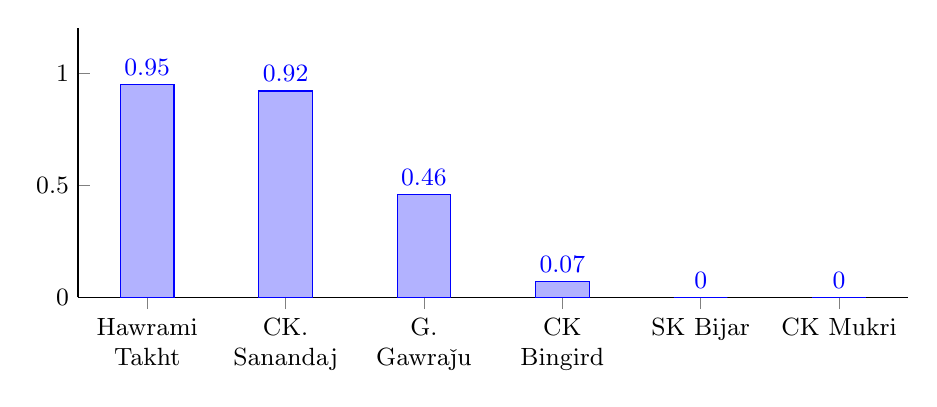
\begin{tikzpicture}
	\small
	\begin{axis}
	  [
		axis lines*=left,
		bar width=5ex,
		font=\small,
		height=5cm,
		enlarge y limits={value=0.2,upper},
		legend cell align=left,
		nodes near coords,
		nodes near coords style={/pgf/number format/fixed},
		width=\textwidth,
		xtick=data,
		symbolic x coords={Hawrami Takht,CK. Sanandaj,G. Gawraǰu,CK Bingird,SK Bijar,CK Mukri},
		x tick label style={text width=1.5cm, align=center, font=\sloppy\small},
		y tick label style={font=\small},
		ybar=3pt,
		ylabel near ticks,
		ymin=0,
		ymax=1
	  ]
	  \addplot coordinates {(Hawrami Takht,0.95) (CK. Sanandaj,0.92) (G. Gawraǰu,0.46) (CK Bingird,0.07) (SK Bijar,0) (CK Mukri,0)};
	\end{axis}
    \end{tikzpicture}
    \caption{Post-predicate ratio of nominal Addressees}
    \label{Kurdish:fig:3}
\end{figure}

The resulting data confirms our hypothesis that the postverbal realisation of nominal Addressees is areally confined to the south of the Central Kurdish speech zone, where we assume a Gorani \isi{substrate}. Interestingly, in the NENA dialect of Sanandaj, Addressee arguments of `say/tell' are 100\% post-predicate \citep[see][]{Noorlander2022WOWAJSana}{}{}, suggesting further that the \isi{word order} profile of Addressees is areally defined. An areally-mediated shift in Addressee placement is also documented for Northern Kurdish in \citet{Haig2022PostPredicateCon}. In the northern Central Kurdish dialects\il{Kurdish (Central)!Bingird} \il{Kurdish (Central)!Mukri} of Mukri and Bingird, the reverse order Addressee-Verb is prevalent, tying in with the ordering in the geographically neighbouring Southern Kurdish Bijar.\il{Kurdish (Southern)!Bijar} 

It is also notable that Central Kurdish Sanandaj\il{Kurdish (Central)!Sanandaj} shows much closer correspondence with the neighbouring Hawrami Takht than with the Kurdicised Gorani Gawraǰu.\il{Gorani!Gawraǰu} The latter is not really a good representative of the original assumed state of, e.g. Gorani as once spoken in Sanandaj, and it is outside of the Central Kurdish region. Indeed, Central Kurdish Sanandaj\il{Kurdish (Central)!Sanandaj} better reflects the original Gorani \isi{word order} than Gorani Gawraǰu.\il{Gorani!Gawraǰu} The real conclusion seems to be the structural proximity of Central Kurdish Sanandaj\il{Kurdish (Central)!Sanandaj} and Hawrami Takht, in line with the assumption of a Gorani \isi{substrate} in Central Kurdish Sanandaj.\il{Kurdish (Central)!Sanandaj}

Relatedly, the opposing directionality in the placement of place arguments of copula construction\is{copula!construction}
s in Central Kurdish Sanandaj\il{Kurdish (Central)!Sanandaj} and Southern Kurdish Bijar\il{Kurdish (Southern)!Bijar} is matched by the same tendencies in immediate neighbouring languages,\footnote{The number of test clauses is 12 for Central Kurdish Mukri,\il{Kurdish (Central)!Mukri} and 10 for Hawrami Takht.} thus in the southern Central Kurdish speech zone place arguments of \isi{copula} verbs are predominantly post-predicate, whereas the reverse ordering holds in the north, see \figref{Kurdish:fig:4}.

\begin{figure}
% % %     \includegraphics[width=\textwidth]{figures/Gorani_fig4.png}\\
    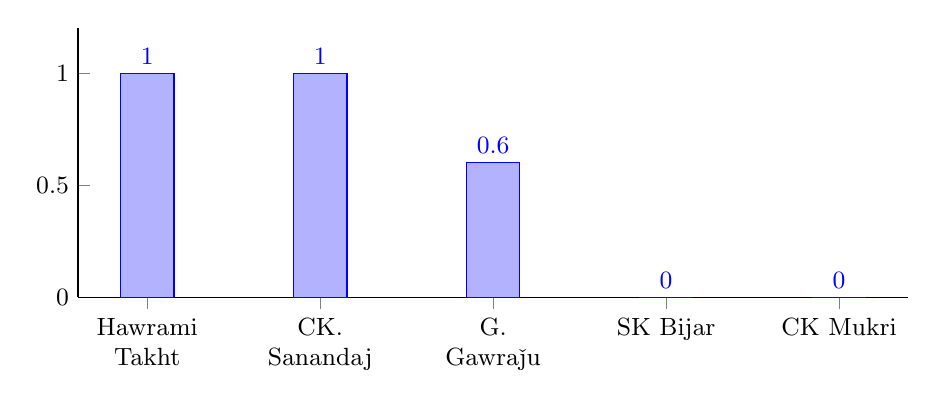
\begin{tikzpicture}
	\small
	\begin{axis}
	  [
		axis lines*=left,
		bar width=5ex,
		font=\small,
		height=5cm,
		enlarge y limits={value=0.2,upper},
		legend cell align=left,
		nodes near coords,
		nodes near coords style={/pgf/number format/fixed},
		width=\textwidth,
		xtick=data,
		symbolic x coords={Hawrami Takht,CK. Sanandaj,G. Gawraǰu,SK Bijar,CK Mukri},
		x tick label style={text width=1.5cm, align=center, font=\sloppy\small},
		y tick label style={font=\small},
		ybar=3pt,
		ylabel near ticks,
		ymin=0,
		ymax=1
	  ]
	  \addplot coordinates {(Hawrami Takht,1) (CK. Sanandaj,1) (G. Gawraǰu,0.6) (SK Bijar,0) (CK Mukri,0)};
	\end{axis}
    \end{tikzpicture}
    \caption{Post-predicate ratio of place constituents in copular constructions}
    \label{Kurdish:fig:4}
\end{figure}

An investigation of these minor \isi{word order} features thus reveals commonalities between southern Central Kurdish dialects, here represented by Central Kurdish Sanandaj\il{Kurdish (Central)!Sanandaj} and Gorani (represented\il{Gorani!Hawrami Takht} by Hawrami Takht). I propose that these differences can be most plausibly explained through the greater influence of Gorani in the southern part of the Central Kurdish speech zone, particularly due to Gorani speakers shifting to Kurdish. Northern Central Kurdish dialects, like Central Kurdish Mukri,\il{Kurdish (Central)!Mukri} in which contact with Gorani was probably not as intense as it was in the south, lack the effects documented here (see \citealt[]{mohammadirad_gorani_inpress}{ for other features which highlight the impact of Gorani \isi{substrate} in creating north/south division of Central Kurdish dialects}). The findings also suggest, conversely, that the remnant Gorani variety of Gawraǰu has diverged from a presumably more conservative state of Hawrami Takht and drawn closer to the more widespread pattern found in Kurdish. 

Note that the minor \isi{word order} patterns considered in this section have generally gone under the radar of the larger-scale approaches to Kurdish \isi{word order} and \isi{language contact} but illustrate the importance of more detailed case studies in identifying local patterns of contact.

\section{Conclusion} \label{MFKC: sec.conc}
Among Iranian languages, Kurdish varieties are the westernmost outlier at the intersection with \isi{VO} languages. This has resulted in the preponderance of \isi{head-initial} \isi{word order} configurations in this group of varieties, as documented in \citet{haig_verb-goal_2015} and subsequent literature. This study highlighted the \isi{word order} profile of \isi{oblique} arguments in three Kurdic dialects, namely Central Kurdish Sanandaj,\il{Kurdish (Central)!Sanandaj} Gorani Gawraǰu,\il{Gorani!Gawraǰu} and Southern Kurdish Bijar.\il{Kurdish (Southern)!Bijar} Major patterns of constituent ordering in these languages match to a large extent; for example, they all have rigid object-\isi{word order}: Goals and nominal Recipients are predominantly postverbal. However, these dialects exhibit microvariation concerning the positioning of Addressees and light-verb complements, and locational copula complement\is{copula!complement}s. These differences were claimed to represent areal patterns and warrant a north-south distinction of Central Kurdish dialects triggered by the Gorani \isi{substrate} in the southern Central Kurdish dialects. It appears that the northern Central Kurdish dialects have preserved the generally assumed Old Iranian pattern of preverbal realisation of Addressees, reinforced through contact with Azeri Turkic\il{Turkic!Azeri} varieties. In \isi{contrast}, the southernmost dialects have shifted to post-verbal Addressees and post-verbal place complements in copula construction\is{copula!construction}s. 

\section*{Abbreviations}
\begin{tabularx}{.5\textwidth}{@{}lQ@{}}
1 & 1st person \\
2 & 2nd person \\
3 & 3rd person \\
A & transitive subject \\
\textsc{adj} 	&adjective \\
\textsc{aux} 	&auxiliary \\
CK & Central Kurdish \\
\textsc{clf}  & classifier \\
\textsc{comp}  &complementizer \\
\textsc{compl} & completive \\
\textsc{cop} & copula \\
\textsc{def} & definite \\
\textsc{deic} & deictic \\ 
\textsc{dem} & demonstrative \\
\textsc{dist} & distal \\
\textsc{drct} & directional particle \\
\textsc{exist} & existential particle \\
\textsc{ez} & ezafe \\
% F& Feminine \\
G  & Gorani \\
\textsc{ind} & indicative \\
\textsc{indf} & indefinite \\
% INF& Infinitive \\
\textsc{ipfv} & imperfective \\ %22
\end{tabularx}%
\begin{tabularx}{.5\textwidth}{@{}lQ@{}}
% M& Masculine \\
\textsc{neg}  & negative \\
\textsc{num} & numeral \\
N& Noun \\
\textsc{obl} & oblique \\
O & Direct Object \\
\textsc{perf} & perfect \\
\textsc{pl} & plural \\
PN& Proper Noun \\
\textsc{pos}  & possessor \\
\textsc{post} & postposition \\
\textsc{proh} & prohibitive \\
\textsc{prox} & proximal \\
\textsc{prs} & present \\
\textsc{pst} & past \\
\textsc{ptcl} & particle \\
\textsc{ptcp} & participle \\
R& Flagged {oblique} {argument}\\
% PVB& Preverb \\
% REFL& Reflexive \\
S & Intransitive Subject \\
\textsc{sbjv} & subjunctive \\
\textsc{sg} & singular \\
SK & Southern Kurdish \\
\textsc{spec} & specific \\
\end{tabularx}

\section*{Acknowledgements}
This research makes a contribution towards (ERC, ALHOME, 101021183). Views and opinions expressed are however those of the author(s) only and do not necessarily reflect those of the European Union or the European Research Council Executive Agency. Neither the European Union nor the granting authority can be held responsible for them. I am very grateful to Geoffrey Haig and Don Stilo for their valuable comments on an earlier draft of this paper. 

% \nocite{HaigKhan2019LLWA}

\sloppy
\printbibliography[heading=subbibliography,notkeyword=this]

\end{sloppypar}
\end{document}
